\documentclass{standalone}
\usepackage{tikz}
\usetikzlibrary{patterns, positioning}


\begin{document}
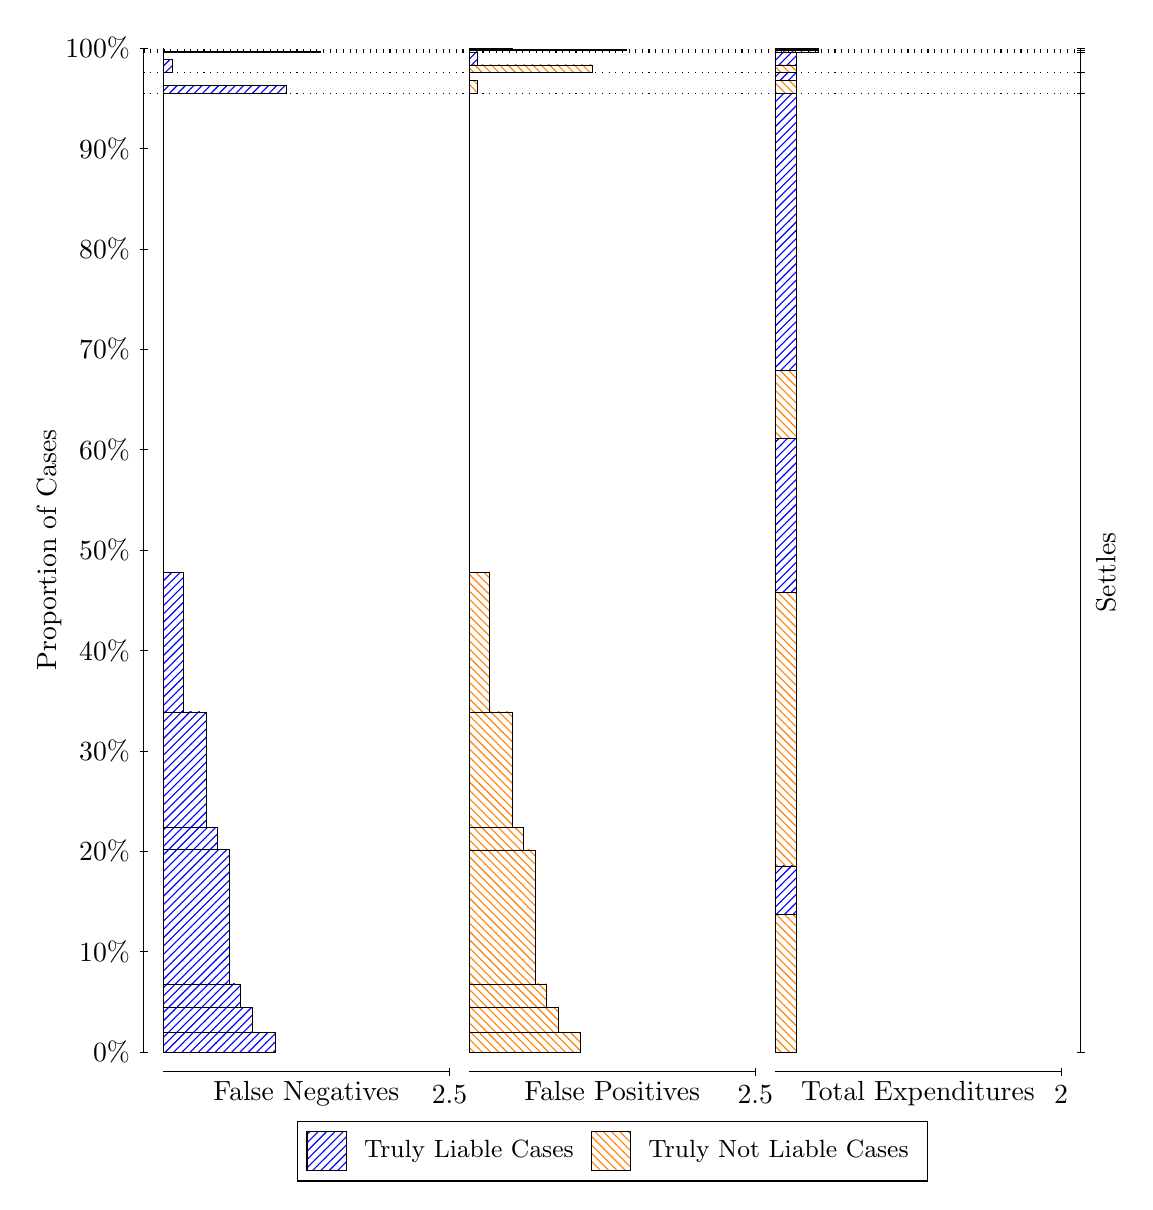
\begin{tikzpicture}
\draw[black, very thin] (1.5,1.75) -- (1.5,14.5);
\node[rotate=90, text=black, anchor=center] at (0.3, 8.125) {Proportion of Cases};
\draw[black, very thin] (1.45,1.75) -- (1.55,1.75);
\node[text=black, anchor=east] at (1.45, 1.75) {0\%};
\draw[black, very thin] (1.45,3.025) -- (1.55,3.025);
\node[text=black, anchor=east] at (1.45, 3.025) {10\%};
\draw[black, very thin] (1.45,4.3) -- (1.55,4.3);
\node[text=black, anchor=east] at (1.45, 4.3) {20\%};
\draw[black, very thin] (1.45,5.575) -- (1.55,5.575);
\node[text=black, anchor=east] at (1.45, 5.575) {30\%};
\draw[black, very thin] (1.45,6.85) -- (1.55,6.85);
\node[text=black, anchor=east] at (1.45, 6.85) {40\%};
\draw[black, very thin] (1.45,8.125) -- (1.55,8.125);
\node[text=black, anchor=east] at (1.45, 8.125) {50\%};
\draw[black, very thin] (1.45,9.4) -- (1.55,9.4);
\node[text=black, anchor=east] at (1.45, 9.4) {60\%};
\draw[black, very thin] (1.45,10.675) -- (1.55,10.675);
\node[text=black, anchor=east] at (1.45, 10.675) {70\%};
\draw[black, very thin] (1.45,11.95) -- (1.55,11.95);
\node[text=black, anchor=east] at (1.45, 11.95) {80\%};
\draw[black, very thin] (1.45,13.225) -- (1.55,13.225);
\node[text=black, anchor=east] at (1.45, 13.225) {90\%};
\draw[black, very thin] (1.45,14.5) -- (1.55,14.5);
\node[text=black, anchor=east] at (1.45, 14.5) {100\%};

\draw[black, very thin] (13.4,1.75) -- (13.4,14.5);
\draw[black, very thin] (13.35,1.75) -- (13.45,1.75);
\node[anchor=west] at (13.35, 1.75) {};
\draw[black, very thin] (13.35,13.928) -- (13.45,13.928);
\node[anchor=west] at (13.35, 13.928) {};
\draw[black, very thin] (13.35,14.189) -- (13.45,14.189);
\node[anchor=west] at (13.35, 14.189) {};
\draw[black, very thin] (13.35,14.45) -- (13.45,14.45);
\node[anchor=west] at (13.35, 14.45) {};
\draw[black, very thin] (13.35,14.475) -- (13.45,14.475);
\node[anchor=west] at (13.35, 14.475) {};
\draw[black, very thin] (13.35,14.5) -- (13.45,14.5);
\node[anchor=west] at (13.35, 14.5) {};

\draw[black, very thin, pattern color=blue, pattern=north east lines] (1.75,1.75) rectangle (3.167,2.0022);
\draw[black, very thin, pattern color=blue, pattern=north east lines] (1.75,2.0022) rectangle (2.8763,2.3201);
\draw[black, very thin, pattern color=blue, pattern=north east lines] (1.75,2.3201) rectangle (2.731,2.6152);
\draw[black, very thin, pattern color=blue, pattern=north east lines] (1.75,2.6152) rectangle (2.5857,4.318);
\draw[black, very thin, pattern color=blue, pattern=north east lines] (1.75,4.318) rectangle (2.4403,4.604);
\draw[black, very thin, pattern color=blue, pattern=north east lines] (1.75,4.604) rectangle (2.295,6.069);
\draw[black, very thin, pattern color=blue, pattern=north east lines] (1.75,6.069) rectangle (2.0043,7.8389);
\draw[black, very thin, pattern color=orange, pattern=north west lines] (1.75,7.8389) rectangle (1.75,13.928);
\draw[black, very thin, pattern color=blue, pattern=north east lines] (1.75,13.928) rectangle (3.3123,14.025);
\draw[black, very thin, pattern color=orange, pattern=north west lines] (1.75,14.025) rectangle (1.75,14.189);
\draw[black, very thin, pattern color=blue, pattern=north east lines] (1.75,14.189) rectangle (1.859,14.353);
\draw[black, very thin, pattern color=orange, pattern=north west lines] (1.75,14.353) rectangle (1.75,14.45);
\draw[black, very thin, pattern color=blue, pattern=north east lines] (1.75,14.45) rectangle (3.7483,14.458);
\draw[black, very thin, pattern color=orange, pattern=north west lines] (1.75,14.458) rectangle (1.75,14.475);
\draw[black, very thin, pattern color=orange, pattern=north west lines] (1.75,14.475) rectangle (1.75,14.483);
\draw[black, very thin, pattern color=blue, pattern=north east lines] (1.75,14.483) rectangle (1.75,14.5);
\draw[black, very thin, pattern color=orange, pattern=north west lines] (5.6333,1.75) rectangle (7.0503,2.0022);
\draw[black, very thin, pattern color=orange, pattern=north west lines] (5.6333,2.0022) rectangle (6.7597,2.32);
\draw[black, very thin, pattern color=orange, pattern=north west lines] (5.6333,2.32) rectangle (6.6143,2.615);
\draw[black, very thin, pattern color=orange, pattern=north west lines] (5.6333,2.615) rectangle (6.469,4.3178);
\draw[black, very thin, pattern color=orange, pattern=north west lines] (5.6333,4.3178) rectangle (6.3237,4.6038);
\draw[black, very thin, pattern color=orange, pattern=north west lines] (5.6333,4.6038) rectangle (6.1783,6.0691);
\draw[black, very thin, pattern color=orange, pattern=north west lines] (5.6333,6.0691) rectangle (5.8877,7.8391);
\draw[black, very thin, pattern color=blue, pattern=north east lines] (5.6333,7.8391) rectangle (5.6333,13.928);
\draw[black, very thin, pattern color=orange, pattern=north west lines] (5.6333,13.928) rectangle (5.7423,14.092);
\draw[black, very thin, pattern color=blue, pattern=north east lines] (5.6333,14.092) rectangle (5.6333,14.189);
\draw[black, very thin, pattern color=orange, pattern=north west lines] (5.6333,14.189) rectangle (7.1957,14.286);
\draw[black, very thin, pattern color=blue, pattern=north east lines] (5.6333,14.286) rectangle (5.7423,14.45);
\draw[black, very thin, pattern color=orange, pattern=north west lines] (5.6333,14.45) rectangle (5.6333,14.467);
\draw[black, very thin, pattern color=blue, pattern=north east lines] (5.6333,14.467) rectangle (5.6333,14.475);
\draw[black, very thin, pattern color=orange, pattern=north west lines] (5.6333,14.475) rectangle (7.6317,14.483);
\draw[black, very thin, pattern color=blue, pattern=north east lines] (5.6333,14.483) rectangle (6.1783,14.5);
\draw[black, very thin, pattern color=orange, pattern=north west lines] (9.5167,1.75) rectangle (9.7892,3.5014);
\draw[black, very thin, pattern color=blue, pattern=north east lines] (9.5167,3.5014) rectangle (9.7892,4.1143);
\draw[black, very thin, pattern color=orange, pattern=north west lines] (9.5167,4.1143) rectangle (9.7892,7.5871);
\draw[black, very thin, pattern color=blue, pattern=north east lines] (9.5167,7.5871) rectangle (9.7892,9.5421);
\draw[black, very thin, pattern color=orange, pattern=north west lines] (9.5167,9.5421) rectangle (9.7892,10.407);
\draw[black, very thin, pattern color=blue, pattern=north east lines] (9.5167,10.407) rectangle (9.7892,13.928);
\draw[black, very thin, pattern color=orange, pattern=north west lines] (9.5167,13.928) rectangle (9.7892,14.092);
\draw[black, very thin, pattern color=blue, pattern=north east lines] (9.5167,14.092) rectangle (9.7892,14.189);
\draw[black, very thin, pattern color=orange, pattern=north west lines] (9.5167,14.189) rectangle (9.7892,14.286);
\draw[black, very thin, pattern color=blue, pattern=north east lines] (9.5167,14.286) rectangle (9.7892,14.45);
\draw[black, very thin, pattern color=orange, pattern=north west lines] (9.5167,14.45) rectangle (10.062,14.467);
\draw[black, very thin, pattern color=blue, pattern=north east lines] (9.5167,14.467) rectangle (10.062,14.475);
\draw[black, very thin, pattern color=orange, pattern=north west lines] (9.5167,14.475) rectangle (10.062,14.483);
\draw[black, very thin, pattern color=blue, pattern=north east lines] (9.5167,14.483) rectangle (10.062,14.5);
\draw[black, dotted] (1.5,13.928) -- (13.4,13.928);
\draw[black, dotted] (1.5,14.189) -- (13.4,14.189);
\draw[black, dotted] (1.5,14.45) -- (13.4,14.45);
\draw[black, dotted] (1.5,14.475) -- (13.4,14.475);
\draw[black, very thin] (1.75,1.5) -- (5.3833,1.5);
\node[text=black, anchor=north] at (3.5667, 1.5) {False Negatives};
\draw[black, very thin] (5.3833,1.45) -- (5.3833,1.55);
\node[text=black, anchor=north] at (5.3833, 1.45) {2.5};

\draw[black, very thin] (5.6333,1.5) -- (9.2667,1.5);
\node[text=black, anchor=north] at (7.45, 1.5) {False Positives};
\draw[black, very thin] (9.2667,1.45) -- (9.2667,1.55);
\node[text=black, anchor=north] at (9.2667, 1.45) {2.5};

\draw[black, very thin] (9.5167,1.5) -- (13.15,1.5);
\node[text=black, anchor=north] at (11.333, 1.5) {Total Expenditures};
\draw[black, very thin] (13.15,1.45) -- (13.15,1.55);
\node[text=black, anchor=north] at (13.15, 1.45) {2};

\node[text=black, centered, rotate=90] at (13.72, 7.839) {Settles};





\draw (7.449999999999999,1.5) node[draw=none] (baseCoordinate) {};
\begin{scope}[align=center]
        \matrix[scale=0.5, draw=black, below=0.5cm of baseCoordinate, nodes={draw}, column sep=0.1cm]{
            \node[rectangle, draw, minimum width=0.5cm, minimum height=0.5cm, pattern color=blue, pattern=north east lines] {}; &
            \node[draw=none, font=\small, text=black] (B) {Truly Liable Cases}; &
            \node[rectangle, draw, minimum width=0.5cm, minimum height=0.5cm, pattern color=orange, pattern=north west lines] {}; &
            \node[draw=none, font=\small, text=black] (B) {Truly Not Liable Cases}; \\
            };
\end{scope}

\end{tikzpicture}
\end{document}